\documentclass{elsarticle}

\journal{Annals of Nuclear Energy}
%%%% packages and definitions (optional)
\newcommand{\Cyclus}{\textsc{Cyclus}\xspace}%
\newcommand{\Cycamore}{\textsc{Cycamore}\xspace}

\usepackage{tabularx}
\usepackage[acronym,toc]{glossaries}
%\newacronym{<++>}{<++>}{<++>}
\newacronym[longplural={metric tons of heavy metal}]{MTHM}{MTHM}{metric ton of heavy metal}
\newacronym{ABM}{ABM}{agent-based modeling}
\newacronym{ACDIS}{ACDIS}{Program in Arms Control \& Domestic and International Security}
\newacronym{ADS}{ADS}{Accelerator-Driven Systems}
\newacronym{AHTR}{AHTR}{Advanced High Temperature Reactor}
\newacronym{ANDRA}{ANDRA}{Agence Nationale pour la gestion des D\'echets RAdioactifs, the French National Agency for Radioactive Waste Management}
\newacronym{ANL}{ANL}{Argonne National Laboratory}
\newacronym{ANS}{ANS}{American Nuclear Society}
\newacronym{API}{API}{application programming interface}
\newacronym{ARE}{ARE}{Aircraft Reactor Experiment}
\newacronym{ARFC}{ARFC}{Advanced Reactors and Fuel Cycles}
\newacronym{ASME}{ASME}{American Society of Mechanical Engineers}
\newacronym{ATWS}{ATWS}{Anticipated Transient Without Scram}
\newacronym{BDBE}{BDBE}{Beyond Design Basis Event}
\newacronym{BIDS}{BIDS}{Berkeley Institute for Data Science}
\newacronym{BWR}{BWR}{Boiling Water Reactors}
\newacronym{CAFCA}{CAFCA}{ Code for Advanced Fuel Cycles Assessment }
\newacronym{CDTN}{CDTN}{Centro de Desenvolvimento da Tecnologia Nuclear}
\newacronym{CEA}{CEA}{Commissariat \`a l'\'Energie Atomique et aux \'Energies Alternatives}
\newacronym{CI}{CI}{continuous integration}
\newacronym{CNEN}{CNEN}{Comiss\~{a}o Nacional de Energia Nuclear}
\newacronym{CNERG}{CNERG}{Computational Nuclear Engineering Research Group}
\newacronym{COSI}{COSI}{Commelini-Sicard}
\newacronym{COTS}{COTS}{commercial, off-the-shelf}
\newacronym{CSNF}{CSNF}{commercial spent nuclear fuel}
\newacronym{CTAH}{CTAHs}{Coiled Tube Air Heaters}
\newacronym{CUBIT}{CUBIT}{CUBIT Geometry and Mesh Generation Toolkit}
\newacronym{CURIE}{CURIE}{Centralized Used Fuel Resource for Information Exchange}
\newacronym{DAG}{DAG}{directed acyclic graph}
\newacronym{DANESS}{DANESS}{Dynamic Analysis of Nuclear Energy System Strategies}
\newacronym{DBE}{DBE}{Design Basis Event}
\newacronym{DESAE}{DESAE}{Dynamic Analysis of Nuclear Energy Systems Strategies}
\newacronym{DHS}{DHS}{Department of Homeland Security}
\newacronym{DOE}{DOE}{Department of Energy}
\newacronym{DRACS}{DRACS}{Direct Reactor Auxiliary Cooling System}
\newacronym{DRE}{DRE}{dynamic resource exchange}
\newacronym{DSNF}{DSNF}{DOE spent nuclear fuel}
\newacronym{DYMOND}{DYMOND}{Dynamic Model of Nuclear Development }
\newacronym{EBS}{EBS}{Engineered Barrier System}
\newacronym{EDF}{EDF}{Électricité de France}
\newacronym{EDZ}{EDZ}{Excavation Disturbed Zone}
\newacronym{EIA}{EIA}{U.S. Energy Information Administration}
\newacronym{EPA}{EPA}{Environmental Protection Agency}
\newacronym{EPR}{EPR}{European Pressurized Reactors}
\newacronym{EP}{EP}{Engineering Physics}
\newacronym{EU}{EU}{European Union}
\newacronym{FCO}{FCO}{Fuel Cycle Options}
\newacronym{FCT}{FCT}{Fuel Cycle Technology}
\newacronym{FEHM}{FEHM}{Finite Element Heat and Mass Transfer}
\newacronym{FEPs}{FEPs}{Features, Events, and Processes}
\newacronym{FHR}{FHR}{Fluoride-Salt-Cooled High-Temperature Reactor}
\newacronym{FLiBe}{FLiBe}{Fluoride-Lithium-Beryllium}
\newacronym{FP}{FP}{Fission Products}
\newacronym{GDSE}{GDSE}{Generic Disposal System Environment}
\newacronym{GDSM}{GDSM}{Generic Disposal System Model}
\newacronym{GENIUSv1}{GENIUSv1}{Global Evaluation of Nuclear Infrastructure Utilization Scenarios, Version 1}
\newacronym{GENIUSv2}{GENIUSv2}{Global Evaluation of Nuclear Infrastructure Utilization Scenarios, Version 2}
\newacronym{GENIUS}{GENIUS}{Global Evaluation of Nuclear Infrastructure Utilization Scenarios}
\newacronym{GPAM}{GPAM}{Generic Performance Assessment Model}
\newacronym{GRSAC}{GRSAC}{Graphite Reactor Severe Accident Code}
\newacronym{GUI}{GUI}{graphical user interface}
\newacronym{HLW}{HLW}{high level waste}
\newacronym{HPC}{HPC}{high-performance computing}
\newacronym{HTC}{HTC}{high-throughput computing}
\newacronym{HTGR}{HTGR}{High Temperature Gas-Cooled Reactor}
\newacronym{IAEA}{IAEA}{International Atomic Energy Agency}
\newacronym{IEMA}{IEMA}{Illinois Emergency Mangament Agency}
\newacronym{IHLRWM}{IHLRWM}{International High Level Radioactive Waste Management}
\newacronym{INL}{INL}{Idaho National Laboratory}
\newacronym{IPRR1}{IRP-R1}{Instituto de Pesquisas Radioativas Reator 1}
\newacronym{IRP}{IRP}{Integrated Research Project}
\newacronym{ISFSI}{ISFSI}{Independent Spent Fuel Storage Installation}
\newacronym{ISRG}{ISRG}{Independent Student Research Group}
\newacronym{JFNK}{JFNK}{Jacobian-Free Newton Krylov}
\newacronym{LANL}{LANL}{Los Alamos National Laboratory}
\newacronym{LBNL}{LBNL}{Lawrence Berkeley National Laboratory}
\newacronym{LCOE}{LCOE}{levelized cost of electricity}
\newacronym{LDRD}{LDRD}{laboratory directed research and development}
\newacronym{LFR}{LFR}{Lead-Cooled Fast Reactor}
\newacronym{LLNL}{LLNL}{Lawrence Livermore National Laboratory}
\newacronym{LMFBR}{LMFBR}{Liquid Metal Fast Breeder Reactor}
\newacronym{LOFC}{LOFC}{Loss of Forced Cooling}
\newacronym{LOHS}{LOHS}{Loss of Heat Sink}
\newacronym{LOLA}{LOLA}{Loss of Large Area}
\newacronym{LP}{LP}{linear program}
\newacronym{LWR}{LWR}{Light Water Reactor}
\newacronym{MAGNOX}{MAGNOX}{Magnesium Alloy Graphie Moderated Gas Cooled Uranium Oxide Reactor}
\newacronym{MA}{MA}{minor actinide}
\newacronym{MCNP}{MCNP}{Monte Carlo N-Particle code}
\newacronym{MILP}{MILP}{mixed-integer linear program}
\newacronym{MIT}{MIT}{the Massachusetts Institute of Technology}
\newacronym{MOAB}{MOAB}{Mesh-Oriented datABase}
\newacronym{MOOSE}{MOOSE}{Multiphysics Object-Oriented Simulation Environment}
\newacronym{MOX}{MOX}{mixed oxide}
\newacronym{MSBR}{MSBR}{Molten Salt Breeder Reactor}
\newacronym{MSRE}{MSRE}{Molten Salt Reactor Experiment}
\newacronym{MSR}{MSR}{Molten Salt Reactor}
\newacronym{NAGRA}{NAGRA}{National Cooperative for the Disposal of Radioactive Waste}
\newacronym{NEAMS}{NEAMS}{Nuclear Engineering Advanced Modeling and Simulation}
\newacronym{NEUP}{NEUP}{Nuclear Energy University Programs}
\newacronym{NFCSim}{NFCSim}{Nuclear Fuel Cycle Simulator}
\newacronym{NGNP}{NGNP}{Next Generation Nuclear Plant}
\newacronym{NMWPC}{NMWPC}{Nuclear MW Per Capita}
\newacronym{NNSA}{NNSA}{National Nuclear Security Administration}
\newacronym{NPRE}{NPRE}{Department of Nuclear, Plasma, and Radiological Engineering}
\newacronym{NQA1}{NQA-1}{Nuclear Quality Assurance - 1}
\newacronym{NRC}{NRC}{Nuclear Regulatory Commission}
\newacronym{NSF}{NSF}{National Science Foundation}
\newacronym{NSSC}{NSSC}{Nuclear Science and Security Consortium}
\newacronym{NUWASTE}{NUWASTE}{Nuclear Waste Assessment System for Technical Evaluation}
\newacronym{NWF}{NWF}{Nuclear Waste Fund}
\newacronym{NWTRB}{NWTRB}{Nuclear Waste Technical Review Board}
\newacronym{OCRWM}{OCRWM}{Office of Civilian Radioactive Waste Management}
\newacronym{ORION}{ORION}{ORION}
\newacronym{ORNL}{ORNL}{Oak Ridge National Laboratory}
\newacronym{PARCS}{PARCS}{Purdue Advanced Reactor Core Simulator}
\newacronym{PBAHTR}{PB-AHTR}{Pebble Bed Advanced High Temperature Reactor}
\newacronym{PBFHR}{PB-FHR}{Pebble-Bed Fluoride-Salt-Cooled High-Temperature Reactor}
\newacronym{PEI}{PEI}{Peak Environmental Impact}
\newacronym{PH}{PRONGHORN}{PRONGHORN}
\newacronym{PRIS}{PRIS}{Power Reactor Information System}
\newacronym{PRKE}{PRKE}{Point Reactor Kinetics Equations}
\newacronym{PSPG}{PSPG}{Pressure-Stabilizing/Petrov-Galerkin}
\newacronym{PWAR}{PWAR}{Pratt and Whitney Aircraft Reactor}
\newacronym{PWR}{PWR}{Pressurized Water Reactor}
\newacronym{PyNE}{PyNE}{Python toolkit for Nuclear Engineering}
\newacronym{PyRK}{PyRK}{Python for Reactor Kinetics}
\newacronym{QA}{QA}{quality assurance}
\newacronym{RDD}{RD\&D}{Research Development and Demonstration}
\newacronym{RD}{R\&D}{Research and Development}
\newacronym{RELAP}{RELAP}{Reactor Excursion and Leak Analysis Program}
\newacronym{RIA}{RIA}{Reactivity Insertion Accident}
\newacronym{RIF}{RIF}{Region-Institution-Facility}
\newacronym{SFR}{SFR}{Sodium-Cooled Fast Reactor}
\newacronym{SINDAG}{SINDA{\textbackslash}G}{Systems Improved Numerical Differencing Analyzer $\backslash$ Gaski}
\newacronym{SKB}{SKB}{Svensk K\"{a}rnbr\"{a}nslehantering AB}
\newacronym{SNF}{SNF}{spent nuclear fuel}
\newacronym{SNL}{SNL}{Sandia National Laboratory}
\newacronym{STC}{STC}{specific temperature change}
\newacronym{SUPG}{SUPG}{Streamline-Upwind/Petrov-Galerkin}
\newacronym{SWF}{SWF}{Separations and Waste Forms}
\newacronym{SWU}{SWU}{Separative Work Unit}
\newacronym{TRIGA}{TRIGA}{Training Research Isotope General Atomic}
\newacronym{TRISO}{TRISO}{Tristructural Isotropic}
\newacronym{TRU}{TRU}{transuranic elements}
\newacronym{TSM}{TSM}{Total System Model}
\newacronym{TSPA}{TSPA}{Total System Performance Assessment for the Yucca Mountain License Application}
\newacronym{ThOX}{ThOX}{thorium oxide}
\newacronym{UFD}{UFD}{Used Fuel Disposition}
\newacronym{UML}{UML}{Unified Modeling Language}
\newacronym{UNF}{UNF}{Used Nuclear Fuel}
\newacronym{UOX}{UOX}{uranium oxide}
\newacronym{UQ}{UQ}{uncertainty quantification}
\newacronym{US}{US}{United States}
\newacronym{UW}{UW}{University of Wisconsin}
\newacronym{VISION}{VISION}{the Verifiable Fuel Cycle Simulation Model}
\newacronym{VVER}{VVER}{Voda-Vodyanoi Energetichesky Reaktor (Russian Pressurized Water Reactor)}
\newacronym{VV}{V\&V}{verification and validation}
\newacronym{WIPP}{WIPP}{Waste Isolation Pilot Plant}
\newacronym{YMR}{YMR}{Yucca Mountain Repository Site}

\makeglossaries
\usepackage{xspace}

\usepackage{caption}
\newcolumntype{b}{X}
\newcolumntype{s}{>{\hsize=.5\hsize}X}
\newcolumntype{m}{>{\hsize=.75\hsize}X}



\usepackage{tikz}
\usetikzlibrary{shapes.geometric,arrows}
\tikzstyle{process} = [rectangle, rounded corners, minimum width=3cm, minimum height=1cm,text centered, draw=black, fill=blue!30]
\tikzstyle{object} = [ellipse, rounded corners, minimum width=3cm, minimum height=1cm,text centered, draw=black, fill=green!30]
\tikzstyle{arrow} = [thick,->,>=stealth]
\usetikzlibrary{positioning, arrows, decorations, shapes }%


\begin{document}
\begin{frontmatter}

\title{Modeling High-fidelity Molten Salt Reactor in a Large-Scale Fuel Cycle Simulation}
\author{Jin Whan Bae$^{1}$, Andrei Rykhlevskii$^{1}$, Benjamin R. Betzler$^{2}$, Joshua L. Peterson-Droogh$^{2}$, Kathryn Huff$^{1}$}
\address{$^{1}$Dept. of Nuclear, Plasma, and Radiological Engineering, University of Illinois at Urbana-Champaign, Urbana, IL \\ $^{2}$Oak Ridge National Laboratory, Oak Ridge, TN }

\begin{abstract}
We developed a method to model \glspl{MSR} in large-scale fuel cycle
simulations by roughly coupling two reactor physics code SERPENT
and SCALE suite of codes. We used Saltproc, an in-house developed
python wrapper to simulate \gls{MSR} behavior in SERPENT. SCALE
has a in-code method of modeling constant addition and removal
of material by editing the Bateman equation. We postprocess the
results from each code to a standardized HDF5 format with
the stream isotopics flow history. We simulated the \gls{MSR}
behavior in \Cyclus, an agent-based simulator, using a \Cyclus archetype
that interprets the HDF5 database that mimics the material flow in and
out of the reactor. This method provides a rapid and high-fidelity
way of modeling \glspl{MSR} in a large-scale fuel cycle simulation.
\end{abstract}

\end{frontmatter}

	

\section{Introduction}

\glspls{MSR} are difficult to model in fuel cycle
simulations due to their continuous reprocessing, where
there is a continuous flow of materials in and out of
the reactors. Many modules have been developed to model
continuous reprocessing in an \gls{MSR}. 



\subsection{\Cyclus}

\Cyclus is an agent-based fuel cycle simulation framework 
\cite{huff_fundamental_2016}, which means 
that each reactor, reprocessing plant, and fuel fabrication plant is modeled as an agent.
A \Cyclus simulation contains prototypes, which are fuel cycle facilities with
pre-defined parameters, that are deployed in the simulation as \texttt{facility} agents.
Encapsulating the \texttt{facility} agents are the \texttt{institution} and \texttt{region}.
A \texttt{region} agent holds a set of \texttt{institution}s.
An \texttt{institution} agent can deploy or decommission \texttt{facility} agents.
The \texttt{institution} agent is part of a \texttt{region} agent,
which can contain multiple \texttt{institution} agents. Several versions of \texttt{Institution}
and \texttt{region} exist, varying in complexity and functions \cite{huff_extensions_2014}.
 \texttt{DeployInst} is used as the institution archetype for this work, where the institution
deploys agents at user-defined timesteps.

At each timestep (one month),
agents make requests for materials or bid to supply them and exchange
with one another. A market-like mechanism called the dynamic resource exchange
\cite{gidden_agent-based_2015} governs the exchanges.
Each material resource has a quantity, composition, name, and a unique identifier
for output analysis. The timestep execution in \Cyclus follows 
\texttt{Build, Tick,} \gls{DRE}, \texttt{Tock, and Decommission}, as illustrated in
figure \ref{fig:time}. The \texttt{Tick}, and \texttt{Tock} phases are for
each agent to perform actions, such as transmutation, separation, or generation
of materials before and after the market exchange phase.

\begin{figure}[h]
\centering
\scalebox{0.7}{
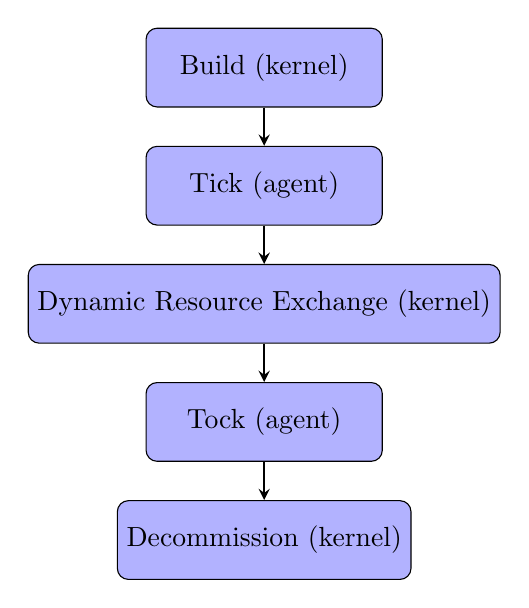
\begin{tikzpicture}[node distance=1.5cm]
\node (Build) [process] {Build (kernel)};
\node (Tick) [process, below of=Build] {Tick (agent)};
\node (DRE) [process, below of=Tick]{Dynamic Resource Exchange (kernel) };
\node (Tock) [process, below of=DRE]{Tock (agent)};
\node (Decom) [process, below of=Tock] {Decommission (kernel)};

\draw [arrow] (Build) -- (Tick); 
\draw [arrow] (Tick) -- (DRE);
\draw [arrow] (DRE) -- (Tock);
\draw [arrow] (Tock) -- (Decom);
\end{tikzpicture}
}
\caption{\Cyclus timestep execution steps.}
\label{fig:time}
\end{figure}

The modularity of \Cyclus allows a low barrier of
entry for developers, since developers can create an
archetype (e.g. Reactor module, Reprocessing module)
without extensive knowledge of the \Cyclus framework.

\subsection{Saltproc}
Saltproc is an external python driver developed to
model batch-wise reprocessing in \glss{MSR}. The code
repeatedly runs SERPENT, performs material operations (e.g. reprocessing,
inflow of fertile material), and saves all material flow
and k-eff values in a HDF5 database. 

\section{Methodology}

[Development of full-core SERPENT MODELS AND OTHER THINGS ANDREI DID]

Then we perform continuous reprocessing analysis on the developed
SERPENT models using Saltproc. The reprocessing scheme is as follows:

[Reprocessing scheme - if different for reactor, mention it]

Note that some reactors have two regions, a driver and a blanket region.
Saltproc is capable of reprocessing from one region and inputting
the separated flow to the other region. For example, plutonium is bred
in the blanket region of a MCSFR, which is separated and input into
the driver region. 

Saltproc also has a reactivity control model, which controls the reactivity
by controlling the amount of fissile material put into the core. At
every depletion step, the k-eff value is checked and modifications
to the fissile stream is made accordingly.


We run the Saltproc for the entire fuel cycle of each \gls{MSR}. For example,
if a \gls{MSR} design asks for a salt-flush (complete unloading of core)
every ten years, the fuel cycle time of the \gls{MSR} would be ten years.
This way, the entire material flow history of the \gls{MSR} is captured
in the Saltproc output database.

The output database is then loaded into the Cyclus module.
The module reads the timestep of the database and the timestep of Cyclus,
and outputs the corresponding waste and surplus fissile stream every timestep.
The module also requests the corresponding amount of fertile material
that the reactor needs from the market. In short, the purpose of the module is to
mimic the interaction of a \gls{MSR} with the market, while producing
power. The module's interaction with the framework is illustrated in
figure \ref{fig:msr_int}.


\begin{figure}[htbp!]
    \begin{center}
        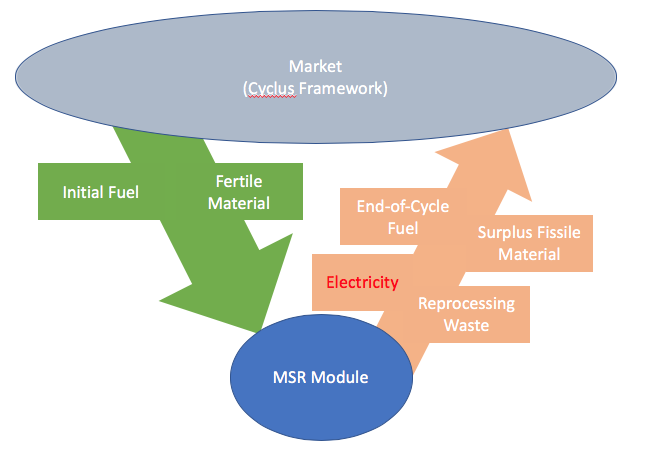
\includegraphics[scale=0.5]{./images/msr_flowchart.png}
    \end{center}
        \caption{Interaction of Cyclus \gls{MSR} module with the Cyclus framework (Market)}
    \label{fig:msr_int}
\end{figure}

\section{Results}

We represent each \Cyclus result as a solid line, and the benchmark solution
as a dotted line for visualization. The results are
simply a reproduction of the plots displayed in the benchmark. 
We obtained the benchmark solutions through personal contact with
benchmark paper's author Bo Feng at Argonne National Laboratory.


Figure \ref{fig:pow_plot} shows the deployed reactor capacity, and
figure \ref{fig:dep} shows the \gls{LWR} retirement and \gls{SFR}
deployment timeseries. The two plots show exact agreement with the
benchmark solutions.

\begin{figure}[htbp!]
	\begin{center}
		\includegraphics[scale=0.5]{./images/results_18/power_plot.png}
	\end{center}
        \caption{Deployed reactor capacities at the end of each year.}
	\label{fig:pow_plot}
\end{figure}



\begin{figure}[htbp!]
	\begin{center}
		\includegraphics[scale=0.5]{./images/results_18/dep.png}
	\end{center}
        \caption{\glspl{LWR} retired and \glspl{SFR} started up each year.}
	\label{fig:dep}
\end{figure}

Figure \ref{fig:fuel_load} shows the annual fuel loading rate.
The initial fuel loading for 100 \gls{LWR} reactors were edited to match
the plot in the verification
study results. Note the oscillations for the \gls{LWR} fuel loading
is caused by the refueling period being 18-month refuel cycle for all \gls{LWR} reactors
aggregated into 12-month groups. Note also that the total values
are equal for both plots.

Although indistinguishable in figure \ref{fig:fuel_load},
there is a small difference with \gls{SFR} fuel loading proportional
to the core mass difference, as mentioned in the previous section.
Figure \ref{fig:fuel_load_diff_norm} shows the
differences normalized by the core mass differences, overlapped with the
\gls{SFR} deployment. This shows that the differences only occur during
deployment due to the difference in core mass.


\begin{figure}[htbp!]
    \begin{center}
        \includegraphics[scale=0.5]{./images/results_18/fuel_load.png}
    \end{center}
        \caption{Annual fresh fuel loading rates (first cores and reload fuel).}
    \label{fig:fuel_load}
\end{figure}

Figure \ref{fig:fuel_discharge_monthly} shows the inventory of discharged
\gls{UNF} in mandatory cooling stage. It also oscillates between the benchmarks
solution,and converges, caused by the influx and the outflux of \gls{UNF}
into and out of the storage facility.
Note that for most plots the \gls{SFR} inventory and fuel loading
exactly matches the benchmark solutions, minus the small difference due to core
size.

\begin{figure}[htbp!]
    \begin{center}
        \includegraphics[scale=0.5]{./images/results_18/fuel_load_diff_norm.png}
    \end{center}
        \caption{Difference of annual fresh \gls{SFR} fuel loading rates (Cyclus - Benchmark) normalized by the core mass difference of an \gls{SFR} due to fractional batch size.}
    \label{fig:fuel_load_diff_norm}
\end{figure}


Figure \ref{fig:waiting_monthly} shows similar results for the inventory of cooled
\gls{UNF} waiting for reprocessing.
Unlike the previous plot, however, the oscillation peaks meet with the benchmark
solution.  This is because the cooled \gls{UNF} inventory is measured by the cumulative sum
of \gls{UNF} that has been cooled subtracted by the \gls{UNF} reprocessed at that timestep.
Thus, the peaks in the oscillation correspond to the cooled inventory in the storage
facility before it sends its inventory to reprocessing.

\begin{figure}[htbp!]
    \begin{center}
        \includegraphics[scale=0.5]{./images/results_18/fuel_discharge_monthly.png}
    \end{center}
        \caption{Inventory of discharged \gls{UNF} in mandatory cooling storage.}
    \label{fig:fuel_discharge_monthly}
\end{figure}


\begin{figure}[htbp!]
    \begin{center}
        \includegraphics[scale=0.5]{./images/results_18/waiting_monthly.png}
    \end{center}
        \caption{Inventory of discharged and cooled \gls{UNF} waiting for reprocessing.}
    \label{fig:waiting_monthly}
\end{figure}


Figure \ref{fig:rep} shows the reprocessing throughput, which also oscillates between
the benchmark solution. Note that no oscillation exists in the beginning because the
\gls{LWR} \gls{UNF} reprocessing plant throughput is maximized at 2,000 tons per year.

\begin{figure}[htbp!]
    \begin{center}
        \includegraphics[scale=0.5]{./images/results_18/rep.png}
    \end{center}
        \caption{Annual reprocessing throughputs.}
    \label{fig:rep}
\end{figure}


Figure \ref{fig:tru} shows the inventory of unused \gls{TRU} recovered from \gls{UNF}.
The \Cyclus results follows the benchmark solutions closely. However, the difference
in core size causes \Cyclus results to be smaller, since more \gls{TRU} is used to
start up the newly deployed \glspl{SFR}. The difference decreases as the
\glspl{SFR} decommission, discharging more \gls{UNF} (thus \gls{TRU}) than
the benchmark.

\begin{figure}[htbp!]
	\begin{center}
		\includegraphics[scale=0.5]{./images/results_18/tru.png}
	\end{center}
        \caption{Inventory of unused \gls{TRU} recovered from \gls{UNF}.}
	\label{fig:tru}
\end{figure}


\section{Discussion}

Leveraging the modularity and agent-based structure of \Cyclus,
we can mimic the fuel cycle impact of \glspl{MSR} using a database
generated from a high-fidelity reactor physics calculation.
This database-approach outsources the computationally heavy
calculations outside the fuel cycle simulation, and allows
for quick, high-resolution implementation of complex systems
in the nuclear fuel cycle.
\section{Acknowledgments}
The work done was funded through the Nuclear
Engineering Science Laboratory Synthesis (NESLS)
program. We thank Eva Davidson from Oak Ridge
National Laboratory (ORNL) and Bo Feng
from Argonne National Laboratory (ANL) for their
aid in providing benchmark solutions and insight
for this work.

\bibliographystyle{elsarticle-num}
\bibliography{bibliography}


\end{document}
